\documentclass[10pt, oneside]{article}
\usepackage{amsmath, amsthm, amssymb, calrsfs, wasysym, verbatim, bbm, color, graphics, graphicx, geometry}
\usepackage[most]{tcolorbox}
\usepackage{xcolor}
\usepackage{framed}
\usepackage{bm}
\usepackage{ragged2e}
\usepackage{amsmath}
\colorlet{shadecolor}{blue!15}
\graphicspath{ {./} }
\geometry{tmargin=.75in, bmargin=.75in, lmargin=.75in, rmargin=.75in}
\newcommand{\R}{\mathbb{R}}
\newcommand{\C}{\mathbb{C}}
\newcommand{\Z}{\mathbb{Z}}
\newcommand{\N}{\mathbb{N}}
\newcommand{\Q}{\mathbb{Q}}
\newcommand{\Cdot}{\boldsymbol{\cdot}}
\newtheorem{thm}{Theorem}
\newtheorem{defn}{Definition}
\newtheorem{conv}{Convention}
\newtheorem{rem}{Remark}
\newtheorem{lem}{Lemma}
\newtheorem{cor}{Corollary}
\newtheorem{exa}{Example}

\title{Clase \# 4: Cinem\'atica de los fluidos [MF100]}
\author{\textbf{Luis Alejandro Morales}\\ \vspace{0.4cm} Profesor Asistente \\ Universidad Nacional de Colombia-Bogot\'a\\Facultad de Ingenier\'ia \\ Departamento de Ingeniería Civil y Agr\'icola}
\date{Periodo 2024-I}

\begin{document}

\maketitle
\tableofcontents

\vspace{.25in}

\section{Descripci\'on Lagrangiana y Euleriana del movimiento de un fluido}

Existen dos aproximaciones para analizar la cinemática de los fluidos. La primera se centra en el análisis de los campos de flujo y es conocido como el método \textbf{Euleriano}. En el método euleriano, se calcula la presión del campo de flujo $p(x,y,z,t)$ (por ejemplo, en un punto del espacio $x,y,z$ o sección), más no los cambios de presión que experimentaría una partícula moviéndose en el flujo. Aquí, la posición del sistema de coordenadas es constante para un intervalo de tiempo (ver Figura~\ref{eulan}). La segunda aproximación se centra en seguir partículas individualmente moviéndose a través del flujo, esto es conocido como el método \textbf{Lagrangiano}. En este, el sistema de coordenadas se mueve con el flujo. El método lagrangiano es más apropiado para el análisis de sólidos, mientras que el método euleriano es ampliamente usado en mecánica de fluidos. En mediciones en fluidos, un sensor de presión introducido en un canal de laboratorio determina la presión del flujo en un punto ($x,y,z$) y en un instante ($t$) determinado. Dicha medición es acorde con el método euleriano. De acuerdo con el método lagrangiano, el mismo sensor arrojado al flujo y moviéndose a la misma velocidad permitiría medir la presión de una partícula que se mueve con el flujo.

\begin{figure}[h]
\centering
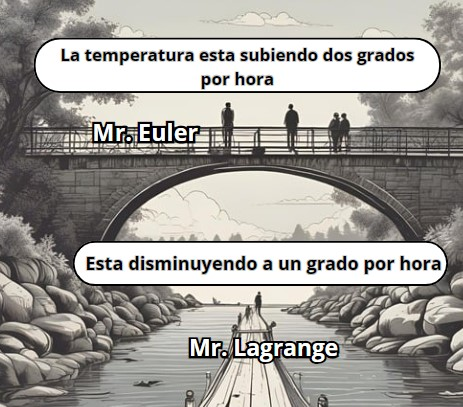
\includegraphics[width=8cm]{Fig.1.jpg}
\caption{Sistema euleriano y lagrangiano}
\label{eulan}
\end{figure}

\subsection{El campo de velocidad}
La propiedad más conocida de un flujo es el campo de velocidad $\vec{V}(x,y,z,t)$, de la cual se derivan otras propiedades. La velocidad es un vector en función de la posición y del tiempo y, por lo tanto, tiene tres componentes escalares $u$, $v$ y $w$:
$$
\vec{V}(x,y,z)=u(x,y,z,t)\vec{i} + v(x,y,z,t)\vec{j} + w(x,y,z,t)\vec{k}
$$

\subsection{El campo de aceleración}
El vector de aceleración, $\vec{a}=\frac{d \vec{V}}{dt}$ es importante en flujos sometidos a algún tipo de fuerza según la segunda ley de Newton. El campo de aceleración de un fluido con respecto a un marco de referencia Euleriano, se define como:
$$
\vec{a}=\frac{d \vec{V}}{dt}
$$

Si tenemos una  $y=f(u)$ donde $u=g(x)$, $y$ es una función compuesta $y=f(g(x))$ y derivable en $x$. De acuerdo con la \textbf{regla de la cadena}, la $\frac{dy}{dx}=\frac{dy}{du} \frac{du}{dx}$. Aplicando dicha regla a la ecuación anterior tenemos: 

$$
\vec{a}=\frac{\partial \vec{V}}{dt} + u\frac{\partial \vec{V}}{dx} + v\frac{\partial \vec{V}}{dy} + w\frac{\partial \vec{V}}{dz}
$$

La aceleración de una partícula de flujo expresada como una variable de campo es:
\begin{equation}
\vec a(x,y,z,t) = \frac{d \vec{V}}{dt} = \frac{\partial \vec{V}}{\partial t} + (\vec{V} \cdot \vec{\nabla})\vec{V}
\label{ace}
\end{equation}

donde $\vec{\nabla}$ es el \emph{operador de gradiente}, el cual se define en coordenadas cartesianas como:
$$
\nabla = \left( \frac{\partial}{\partial x} , \frac{\partial}{\partial y}, \frac{\partial}{\partial z} \right) = \vec{i}\frac{\partial}{\partial x} +\vec{j}\frac{\partial}{\partial y}  + \vec{k}\frac{\partial}{\partial z}
$$

Las componentes de vector de aceleración en coordenadas cartesianas son:
$$
a_x = \frac{\partial u}{\partial t} + u\frac{\partial u}{\partial x} + v\frac{\partial u}{\partial y} + w\frac{\partial u}{\partial z} \\
a_y = \frac{\partial v}{\partial t} + u\frac{\partial v}{\partial x} + v\frac{\partial v}{\partial y} + w\frac{\partial v}{\partial z} \\ 
a_z = \frac{\partial w}{\partial t} + u\frac{\partial w}{\partial x} + v\frac{\partial w}{\partial y} + w\frac{\partial w}{\partial z}  
$$

En la ecuación~\ref{ace}, el término $\partial \vec{V}/\partial t$ es conocida como la \emph{aceleración local} y es diferente de cero para flujo no permanente. El segundo término, $(\vec{V} \cdot \vec{\nabla})\vec{V}$ es conocido como la \emph{aceleración advectiva} o la \emph{aceleración convectiva}. Esto último explica el movimiento de las partículas (advección o convección) de una localización hacia otra en el fluido, donde el campo de velocidades del fluido es diferente. Por ejemplo, consideremos la salida de agua de una manguera cuyo orificio de salida se reduce gradualmente (ver figura~\ref{acel}). En el sistema Euleriano, el flujo es considerado permanente, ya que las propiedades del flujo en cualquier punto del flujo no cambian con el tiempo. Sin embargo, las partículas cambian de velocidad y se aceleran a la salida de la manguera en la reducción gradual. Por lo tanto, la aceleración no es cero debido al término de aceleración advectiva en la ecuación~\ref{ace}. Se puede concluir que el flujo puede ser considerado \emph{permanente} desde un marco de referencia \emph{Euleriano} y \emph{no permanente} desde un marco de referencia \emph{Lagrangiano} que se mueve con el fluido.

% Fig 4-8 Cengel 
\begin{figure}[h]
\centering
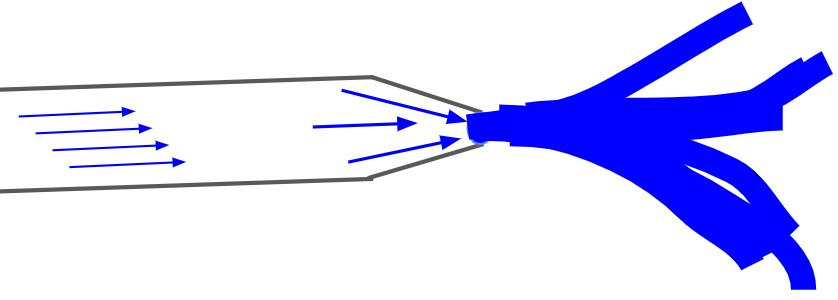
\includegraphics[width=8cm]{Fig.2.jpg}
\caption{Flujo a la salida de una manguera cuyo orificio se reduce y acelera el flujo a la salida.}
\label{acel}
\end{figure}

\subsection{Derivada material}
El operador de derivada total $d/dt$ en la ecuación~\ref{ace} es conocido como la \emph{derivada material}, $D/Dt$ la cual se deduce al seguir una partícula que se mueve con el campo de flujo. La derivada material se expresa como:
\begin{equation}
\underbrace{\frac{D}{Dt}}_{\substack{\text{Material} \\ \text{derivative}}} = \frac{d}{dt} = \underbrace{\frac{\partial}{\partial t}}_{\text{Local}} + \underbrace{(\vec{V} \cdot \vec{\nabla})}_{\text{Advective}}
\label{dma}
\end{equation}
Aplicando la ecuación~\ref{dma} al campo de velocidades tenemos que $\frac{D\vec{V}}{Dt} = \frac{d\vec{V}}{dt}$ y se obtiene la ecuación~\ref{ace}, conocida también como la \emph{aceleración material}.

La ecuación~\ref{dma} puede ser aplicada a variables escalares como la presión:
$$
\frac{DP}{Dt}=\frac{dP}{dt}=\frac{\partial P}{\partial t} + (\vec{P} \cdot \vec{\nabla})\vec{V}
$$
la cual representa la tasa de cambio de la presión  de una partícula que se mueve con el campo del flujo.

\section{Patrones de flujo}

\subsection{Líneas de flujo}

Una \textbf{línea de flujo} es una curva que es tangente al vector de velocidad local en un instante de tiempo. Las líneas de flujo indican la dirección instantánea del movimiento del flujo. Esto quiere decir que en \emph{flujo no permanente} las líneas de flujo cambian con el tiempo. Si consideramos una longitud de arco infinitesimal $d\vec{r}=dx\vec{i}+dy\vec{j}+dz\vec{k}$ a lo largo de una línea de flujo donde $d\vec{r}$ es paralela al vector de velocidad local $\vec{V}=u\vec{i}+v\vec{j}+w\vec{k}$, por similitud de triángulos $d\vec{r}$ debe ser proporcional a $\vec{V}$ (ver figura~\ref{strl}):

$$
\frac{dr}{V}=\frac{dx}{u}=\frac{dy}{v}=\frac{dz}{w}
$$

donde $dr$ es la magnitud de $d\vec{r}$ y $V$ es la magnitud de $\vec{V}$. En el plano $xy$, $(x,y)$, $(u,v)$, la siguiente ecuación se obtiene: 

\begin{equation}
\left(\frac{dy}{dx}\right)_{\text{a lo largo de la línea de flujo}} = \frac{v}{u}
\label{lnf}
\end{equation}

Conociendo el campo de velocidades, la ecuación~\ref{lnf} puede ser resuelta, analítica o numéricamente, pero en cualquier caso una constante de integración es necesaria, lo que daría lugar a una familia de curvas (líneas de flujo).

% Fig 4-16 Cengel 
\begin{figure}[h]
\centering
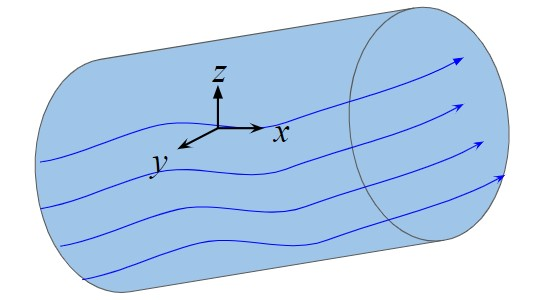
\includegraphics[width=8cm]{Fig.3.jpg}
\caption{Línea de flujo y velocidad instantánea local en tres dimensiones.}
\label{strl}
\end{figure}

\subsection{Trayectorias de corriente}

Una \textbf{trayectoria de corriente} es la trayectoria de viaje de una partícula de fluido durante un período de tiempo siguiendo el método \emph{Lagrangiano}. La trayectoria de corriente está determinada por el vector posición de una partícula ($x(t),\ y(t),\ z(t)$) para un período de tiempo (ver figura~\ref{pathl}). La trayectoria de corriente para un campo de velocidades conocido puede ser calculada como:



\begin{equation}
\vec{x} = \vec{x}_{\text{start}} + \int_{t_{\text{start}}}^t \vec{V} dt
\label{patl}
\end{equation}

donde $x_{\text{start}}$ es la posición inicial de la partícula trazadora en el tiempo inicial $t_{\text{start}}$. Si el campo de velocidades es permanente, las partículas de fluido siguen las líneas de flujo y estas son idénticas a las trayectorias de corriente.

\emph{Particle image velocimetry (PIV)} es una técnica para medir la velocidad de un campo de flujo. PIV usa pequeñas partículas suspendidas en el flujo como trazadores, las cuales son iluminadas con luz láser para determinar la posición y dirección de cada una de ellas en un instante de tiempo.

% Fig 4-20 Cengel 
\begin{figure}[h]
\centering
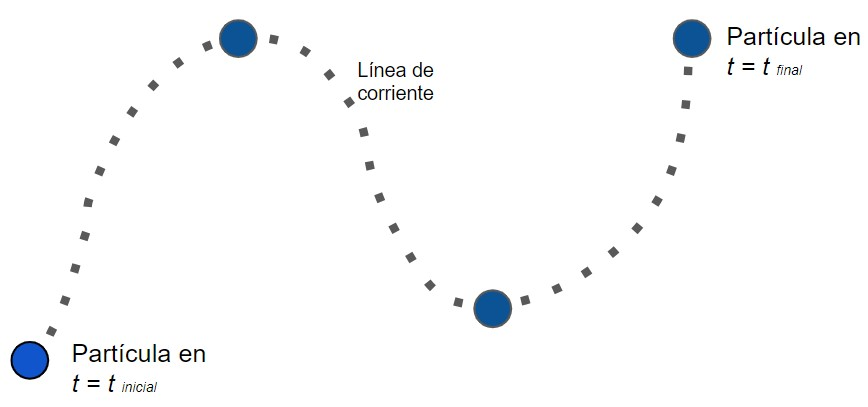
\includegraphics[width=8cm]{Fig.4.jpg}
\caption{Trayectoria de corriente de una partícula.}
\label{pathl}
\end{figure}

\subsection{Líneas de trazos}

Si insertamos un pequeño tubo dentro de un fluido e introducimos un trazador continuo dentro del fluido, la curva que forma las diferentes partículas trazadoras liberadas en intervalo de tiempo constante son la \textbf{línea de trazos} (ver figura~\ref{litra}). Note que en la figura~\ref{litra}, el número sobre la partícula indica el orden en que fueron liberadas dentro del fluido.

% Fig 4-23 Cengel 
\begin{figure}[h]
\centering
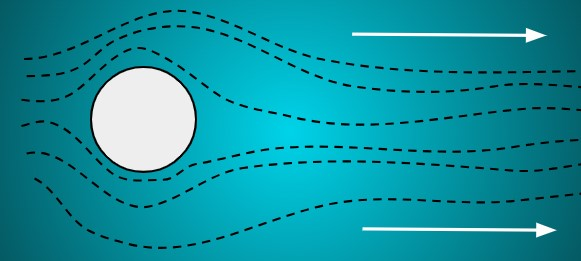
\includegraphics[width=8cm]{Fig.5.jpg}
\caption{Línea de trazos formada por la inyección continua de un trazador en un fluido.}
\label{litra}
\end{figure}

Mientras que en \emph{flujo permanente}, las \emph{líneas de flujo}, las \emph{trayectorias de corriente} y las \emph{líneas de trazos} son iguales, en \emph{flujo no permanente} estas no coinciden. La principal diferencia es que las líneas de flujo son patrones instantáneos de flujo, mientras que las líneas de trazos es una foto del patrón promedio del flujo en un intervalo de tiempo y las trayectorias de corriente son el recorrido de una partícula en un intervalo de tiempo.


% WE NEED VIDEOS TO EXPLAIN THE DIFERENCES

En un campo de flujo conocido, la línea de trazos puede conocerse a partir de la inyección continua de un trazador en un fluido desde un tiempo inicial de la inyección $t_{\text{inject}}$ hasta un tiempo actual $t_{\text{present}}$ utilizando la ecuación~\ref{patl} de la siguiente manera:

\begin{equation}
\vec{x} = \vec{x}_{\text{injection}} + \int_{t_{\text{inject}}}^{t_{\text{present}}} \vec{V} dt
\label{trazl}
\end{equation}

\subsection{Líneas de tiempo}

Las \textbf{líneas de tiempo} son representadas por partículas adyacentes para $t_0$ cuya línea se va deformando a lo largo del flujo gracias al campo de velocidades y la fricción con las paredes. Estas son importantes para examinar la uniformidad del flujo. 

% Fig 4-28 Cengel 
\begin{figure}[h]
\centering
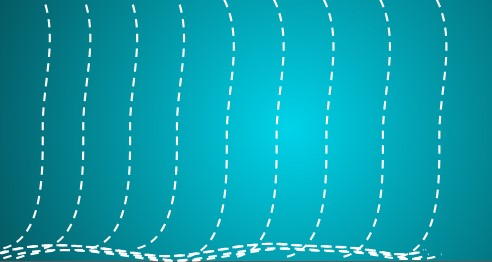
\includegraphics[width=8cm]{Fig.6.jpg}
\caption{Línea de tiempo formada por partículas que se deforma en el tiempo debido al campo de flujo.}
\label{linet}
\end{figure}

\section{Tipos de movimiento o deformación de un elemento de fluido}

Un elemento de fluido puede estar sometido a cuatro tipos de movimiento o deformación: \textbf{traslación}, \textbf{rotación}, \textbf{deformación lineal} y \textbf{deformación cortante} (ver figura~\ref{tmove}). El estudio de la dinámica de fluidos es complicado, ya que estos tipos de movimiento ocurren muchas veces simultáneamente. Estos tipos de movimiento son descritos en términos de tasas (en matemáticas, velocidad y sus derivadas): \emph{velocidad} (tasa de traslación), \emph{velocidad angular} (tasa de rotación), \emph{tasa de deformación lineal}, \emph{tasa de deformación cortante}.

% Fig 4-35 Cengel 
\begin{figure}[h]
\centering
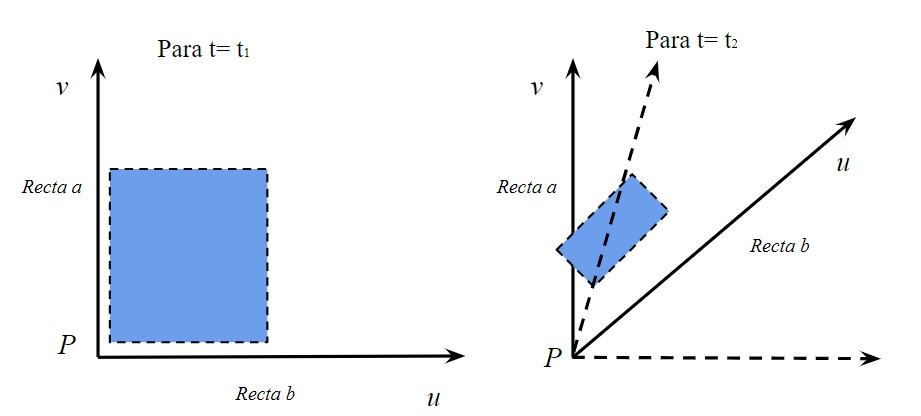
\includegraphics[width=8cm]{Fig.10.jpg}
\caption{Tipos de movimiento: fluido sometido a rotación, deformación cortante o traslación}
\label{tmove}
\end{figure}

\begin{enumerate}
    \item \textbf{Traslación:}
        \begin{equation}
            \text{Variación de posición: } \frac{d\mathbf{r}}{dt} = \mathbf{u}
        \end{equation}

    \item \textbf{Rotación:}
        \begin{equation}
            \text{Variación angular: } \frac{d\theta}{dt} = \omega
        \end{equation}

    \item \textbf{Deformación Lineal:}
        \begin{equation}
            \text{Deformación lineal en una dirección: } \varepsilon = \frac{\Delta L}{L_0}
        \end{equation}

    \item \textbf{Deformación Cortante:}
        \begin{equation}
            \text{Deformación cortante: } \gamma = \tan(\phi) = \frac{\Delta x}{h}
        \end{equation}
\end{enumerate}
\subsection{Velocidad}

La velocidad en un punto se define como la tasa de traslación de dicho punto. Consideremos la figura 7, donde un elemento en 2D se traslada y rota. En el tiempo $t_1$, el punto $P$ tiene coordenadas $(x, y)$. Después de un intervalo de tiempo $dt=t_2 - t_1$, el punto $P$ se ha trasladado a nuevas coordenadas $(x + \Delta x, y + \Delta y)$.

La velocidad $\mathbf{u}$ se define como el vector de traslación promedio por unidad de tiempo:

\[
\mathbf{u} = \frac{d\mathbf{r}}{dt} = \begin{bmatrix} \frac{\Delta x}{dt} \\ \frac{\Delta y}{dt} \end{bmatrix} = \begin{bmatrix} u \\ v \end{bmatrix}
\]

\subsection{Velocidad angular}

La velocidad angular en un punto se define como la tasa de rotación promedio de dos líneas perpendiculares que se intersecan en dicho punto. Consideremos la figura~\ref{rotat} donde un elemento en 2D rota, se traslada y se deforma. En el tiempo $t_1$, las líneas $a$ y $b$ se intersecan perpendicularmente en el punto $P$ en el plano $xy$. Cuando el elemento se mueve y rota en un intervalo $dt=t_2 - t_1$, en el tiempo $t_2$ la línea $a$ rota un ángulo $\alpha_a$ y la línea $b$ rota $\alpha_b$, ambos ángulos son positivos porque rotan en contra de las manecillas del reloj. El ángulo promedio de rotación en $dt$ es, por lo tanto, $(\alpha_a + \alpha_b)/2$. La tasa de rotación o velocidad angular $\omega$ es entonces la derivada con respecto a $t$ del ángulo promedio como:

\[
\omega = \frac{d}{dt}\left( \frac{\alpha_a + \alpha_b}{2} \right) = \frac{1}{2} \left( \frac{\partial v}{\partial x} - \frac{\partial u}{\partial y} \right)
\]

\subsection{Tasa de Deformación Lineal}

La tasa de deformación lineal en un punto se define como la tasa de cambio de la deformación en ese punto. Consideremos la figura 7, donde un elemento en 2D se deforma y rota. En el tiempo $t_1$, el elemento tiene una longitud original $L_0$. Después de un intervalo de tiempo $dt=t_2 - t_1$, la longitud del elemento cambia a $L$.

La tasa de deformación lineal $\dot{\varepsilon}$ se define como la variación relativa de longitud por unidad de tiempo:

\[
\dot{\varepsilon} = \frac{1}{L_0} \frac{dL}{dt}
\]

Esta tasa de deformación lineal también puede expresarse en términos de las derivadas parciales de las componentes de velocidad:

\[
\dot{\varepsilon} = \frac{1}{2} \left( \frac{\partial u}{\partial x} + \frac{\partial v}{\partial y} \right)
\]

\subsection{Tasa de Deformación Cortante}

La tasa de deformación cortante en un punto se define como la tasa de cambio de la deformación cortante en ese punto. Consideremos la figura 8, donde un elemento en 2D se somete a deformación cortante. En el tiempo $t_1$, las líneas $c$ y $d$ son originalmente perpendiculares. Después de un intervalo de tiempo $dt=t_2 - t_1$, debido a la deformación cortante, las líneas $c$ y $d$ ya no son perpendiculares.

La tasa de deformación cortante $\dot{\gamma}$ se define como el cambio angular relativo de las líneas $c$ y $d$ por unidad de tiempo:

\[
\dot{\gamma} = \frac{1}{2} \left( \frac{\partial v}{\partial x} + \frac{\partial u}{\partial y} \right)
\]


% Fig 4-36 Cengel 

\begin{figure}[h]
\centering
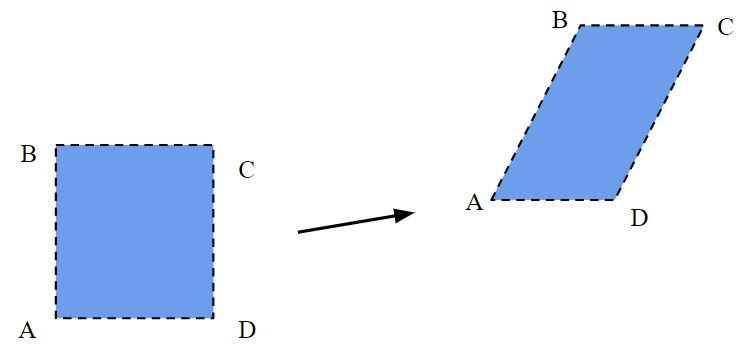
\includegraphics[width=8cm]{Fig.11.jpg}
\caption{Rotación, traslación y deformación de un elemento de fluido en 2D.  Rotación en el punto $P$.}
\label{rotat}
\end{figure}

\section{Clasificación de los flujos}

Como consecuencia de las propiedades de un fluido, el estudio del flujo se deriva de la variación en el tiempo y el espacio para una configuración específica. A su vez, está determinado por las dimensiones efectivas del flujo según el campo de aplicación, es posible caracterizar un flujo basándonos en tres principios fundamentales: variaciones en el tiempo, variaciones en el espacio y características asociadas a su viscosidad (como el número de Reynolds). También podemos incluir su respectivo análisis en unidimensionalidad, bidimensionalidad o tridimensionalidad.

\subsection{Flujo Laminar}

El \textbf{flujo laminar} El flujo laminar en mecánica de fluidos se hace referencia al movimiento ordenado y suave de un fluido, caracterizado por capas no alteradas que se desplazan de manera uniforme. Este fenómeno se observa típicamente en fluidos con viscosidad significativa y a bajas velocidades. El flujo laminar puede modelarse utilizando la ecuación de Navier-Stokes, que describe la conservación de la cantidad de movimiento en un fluido. En el caso del flujo laminar, las soluciones a estas ecuaciones muestran perfiles de velocidad definidos. Para esta caracterizar este estado se tiene que el número de Reynolds ($Re$) es bajo ($Re < 2000$).

\begin{figure}[h]
\centering
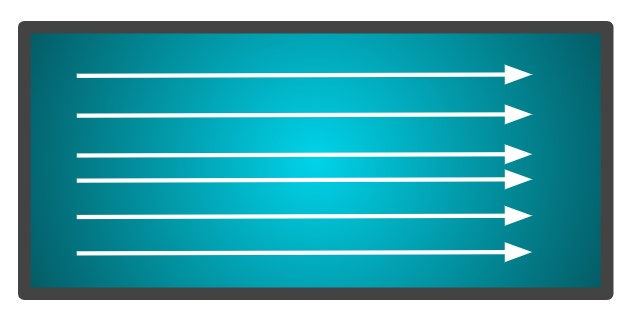
\includegraphics[width=8cm]{Fig.7.jpg}
\caption{Flujo laminar.}
\label{tmove}
\end{figure}

\subsection{Flujo Turbulento}

En el \textbf{flujo turbulento} corresponde a un movimiento desordenado y caótico del fluido, caracterizado por fluctuaciones turbulentas que mezclan las capas presentadas en un flujo laminar, se manifiesta comúnmente a altas velocidades y en fluidos con baja viscosidad. El modelo matemático principal para describir el flujo turbulento es la ecuación de Navier-Stokes, pero en este caso, las soluciones son mucho más complejas debido a la presencia de términos no lineales y fluctuaciones turbulentas. La expresión general de las ecuaciones de Navier-Stokes tenemos: 

\[ \frac{\partial \mathbf{u}}{\partial t} + (\mathbf{u} \cdot \nabla)\mathbf{u} = -\frac{1}{\rho}\nabla p + \nu \nabla^2 \mathbf{u} - \frac{\rho}{2}(\nabla \mathbf{u})^2 + \mathbf{f} \]

Donde:
\begin{itemize}
  \item $\mathbf{u}$ es el vector de velocidad del fluido.
  \item $t$ es el tiempo.
  \item $\rho$ es la densidad del fluido.
  \item $p$ es la presión del fluido.
  \item $\nu$ es la viscosidad cinemática del fluido.
\end{itemize} 

Este tipo de flujo se asocia comúnmente con valores altos de Reynolds ($Re > 4000$ para una tubería circular).

\begin{figure}[h]
\centering
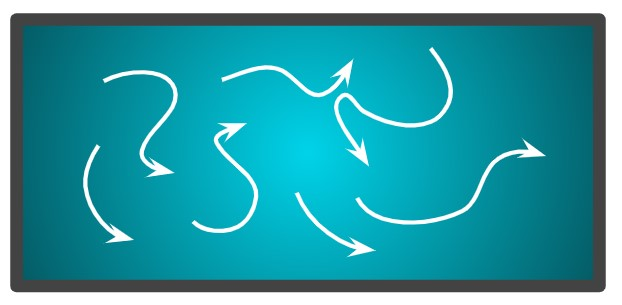
\includegraphics[width=8cm]{Fig.8.jpg}
\caption{Flujo turbulento.}
\label{tmove}
\end{figure}


\subsection{Flujo Compresible}

En el \textbf{flujo compresible}, la densidad del fluido varía significativamente, y se deben considerar las ecuaciones de flujo compresible para describir su comportamiento.

\[
\frac{\partial \rho}{\partial t} + \nabla \cdot (\rho \mathbf{V}) + \rho(\nabla \cdot \mathbf{V}) = 0
\]

\subsection{Número de Reynolds}

El \textbf{número de Reynolds} ($Re$) es una variable adimensional que caracteriza el tipo de flujo en un sistema. Se define como:

\[
Re = \frac{\rho V L}{\mu}
\]

donde $\rho$ es la densidad del fluido, $V$ es la velocidad característica, $L$ es la longitud característica o de sección, y $\mu$ es la viscosidad dinámica. Es ampliamente usado para caracterizar el tipo de flujo según su régimen, especialmente en tuberías, su deducción se atribuye a los experimentos de Osborne Reynolds. Según lo anterior, un flujo puede clasificarse como \textbf{turbulento, de transición o laminar}


\section{Teorema de transporte de Reynolds}
Para establecer el vínculo entre el enfoque de un sistema y un volumen de control aparece el RTT (por sus siglas en inglés). Este teorema lleva el nombre del ingeniero inglés Osborne Reynolds, quien contribuyó significativamente a su aplicación en la mecánica de fluidos. La formulación general del RTT se puede derivar para sistemas con formas e interacciones arbitrarias, pero esta deducción es bastante complicada. Para comprender su significado fundamental, se sugiere inicialmente obtenerla directamente utilizando una configuración geométrica simple antes de generalizar los resultados.

%Insertar figura% 

La ecuación simplificada del teorema de Transporte de Reynolds es:

\begin{equation}
    \frac{d}{dt}B = \underbrace{\frac{dB}{dt}\Bigr|_{\text{VC}}}_{\substack{\text{Tasa de cambio de } B \\\text{respecto al tiempo del volumen de control}}} + \underbrace{\dot{m}_B}_{\substack{\text{Flujo neto de } B \\\text{a través de la superficie de control}}}
\end{equation}

Es importante considerar que para un volumen finito el análisis de la propiedad dentro de él (ya sea intensiva o extensiva) está descrito por la derivada material del mismo:

\begin{equation}
\frac{D}{Dt}B = \frac{\partial B}{\partial t} + (\mathbf{V} \cdot \nabla)B
\end{equation}

La aplicación más general del teorema se resume a evaluar como cambia un fluido respecto a su propiedad interna dentro del volumen de control, así como el flujo existente permiten las entradas y salidas en el sistema.
Para el caso donde se considera esto último, la tasa de cambio temporal para una propiedad en el sistema se expresa como: 

\begin{equation}
    \frac{d}{dt}B = \underbrace{\frac{dB}{dt}\Bigr|_{\text{VC}}}_{\substack{\text{Tasa de cambio de } B \\\text{respecto al tiempo del volumen de control}}} + \underbrace{\dot{m}_B}_{\substack{\text{Flujo neto de } B \\\text{a través de la superficie de control}}} + \underbrace{B_{\text{in}}}_{\substack{\text{Entrada de } B \\\text{al sistema}}} - \underbrace{B_{\text{out}}}_{\substack{\text{Salida de } B \\\text{del sistema}}}
\end{equation}

\begin{figure}[h]
\centering
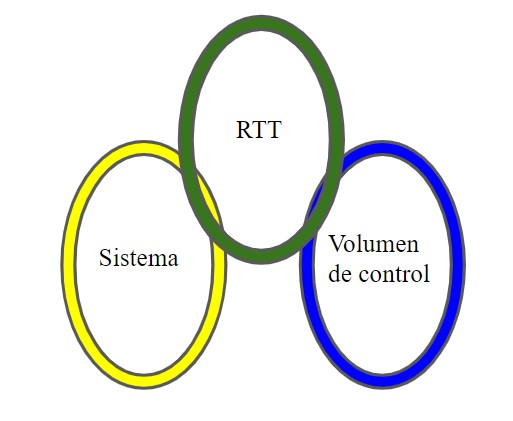
\includegraphics[width=7cm]{Fig.9.jpg}
\caption{Relación RTT.}
\label{tmove}
\end{figure}\textbf{}

\subsection{Sistemas cerrados y abiertos}

Para poder evaluar los problemas habituales de la mecánica de fluidos es importante trabajar con un volumen de control, el cual se define como una región en el espacio elegida para su estudio. Dependiendo de si la masa interna de dicho sistema es capaz de salir o no, estaremos hablando de sistemas cerrados o abiertos, nótese que la elección de este volumen es arbitraria y fija respecto al sistema que se analiza, pero se recomienda una adecuada delimitación para la solución del problema.

En su mayoría, los problemas de la materia se trabajan para sistemas abiertos donde la masa es capaz de entrar o salir por superficies de control, esto significa que el volumen de dicho sistema permanecerá constante mientras que su masa (la cual puede entrar o salir por dichas superficies) puede ser variable, las superficies a diferencia del volumen de control pueden deformarse o desplazarse 

%Inssertar ejemplos%

\subsection{Fuerzas actuantes sobre un volumen de control}

Para el volumen de control escogido, el análisis de fuerzas considera todas las componentes a las cuales está sometido, tanto aquellas que actúan sobre todo lo encerrado en dicho volumen (gravedad, eléctrica y magnética), y las fuerzas superficiales propias al tipo de problema, un ejemplo de la misma es la viscosidad, también se deben tomar en cuenta las fuerzas de reacción en los puntos de contacto. En el análisis del volumen de control, la suma de todas estas fuerzas que actúan sobre el volumen de control en un instante en particular, se representa por \textbf{F} y se expresa como: 

\begin{equation}
\sum \vec{\mathbf{F}} = \sum \vec{\mathbf{F}}{\text{cuerpo}} + \sum \vec{\mathbf{F}}{\text{superficial}}
\end{equation}

%\documentclass{article}
%\usepackage{amsmath}
%\usepackage{bm}
%
%\begin{document}

\section{Ecuación de continuidad}
A través de la aplicación del teorema de transporte de Reynolds, se tiene la expresión general para la conservación de masa:

\begin{equation}
\frac{\partial}{\partial t} \int_{VC} \rho  dV + \int_{SC} \rho (\mathbf{\vec{V}} \cdot \mathbf{\vec{n}}) dA = 0
\end{equation}

\subsection{Ecuación de continuidad para un caso general}
Siempre y cuando la velocidad sea absoluta, esta ecuación funciona para volúmenes de control fijos o móviles, dicha ecuación en términos de superficies de control para la entrada y la salida fijos puede ser reescrita como: 

\begin{equation}
\frac{\partial}{\partial t} \int_{VC}\rho dV= \sum_{\text{ent}} \dot{\bm{m}} - \sum_{\text{sal}}\dot{\bm{m}}
\end{equation}

\begin{figure}[h]
\centering
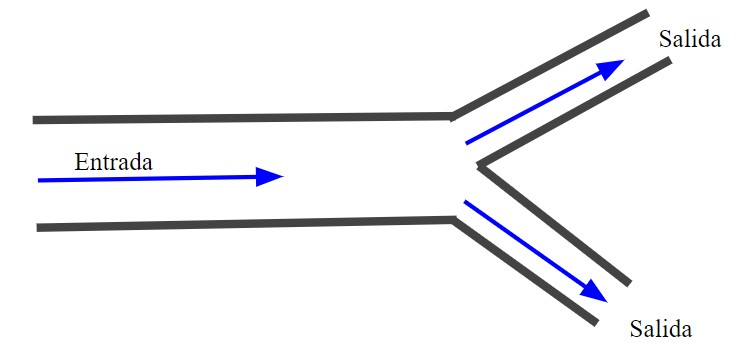
\includegraphics[width=8cm]{Fig.12.jpg}
\caption{Continuidad: caso de una tubería.}
\label{tmove}
\end{figure}

La simplificación de esta ecuación indica que la razón de cambio de masa dentro del volumen de control es igual a la razón a la que fluye la masa hacia el "interior" del volumen de control, menos la razón a la que fluye la masa "afuera" del volumen de control. Nótese que esta expresión aplica para cualquier volumen de control sin importar su tamaño.

Además, para un volumen de control diferencial (considerando una extensión infinitamente pequeña), la ecuación de continuidad se puede expresar en forma local como:

\begin{equation}
\frac{\partial \rho}{\partial t} + \nabla \cdot (\rho \mathbf{\vec{V}}) = 0
\end{equation}

Esta forma diferencial de la ecuación de continuidad establece que la tasa de cambio temporal de la densidad $\rho$ en un punto más la divergencia del flujo de masa es cero. Es una expresión que asegura la conservación de la masa en un fluido, indicando que cualquier cambio en la densidad en un punto es compensado por el flujo de masa hacia o desde ese punto.
\end{document}

